\documentclass[journal]{IEEEtran}
\usepackage[a5paper, margin=10mm, onecolumn]{geometry}
\usepackage{tfrupee} % Include tfrupee package

\setlength{\headheight}{1cm} % Set the height of the header box
\setlength{\headsep}{0mm}     % Set the distance between the header box and the top of the text

\usepackage{gvv}
\usepackage{cite}
\usepackage{amsmath,amssymb,amsfonts,amsthm}
\usepackage{algorithmic}
\usepackage{graphicx}
\usepackage{textcomp}
\usepackage{xcolor}
\usepackage{txfonts}
\usepackage{listings}
\usepackage{enumitem}
\usepackage{mathtools}
\usepackage{gensymb}
\usepackage{comment}
\usepackage[breaklinks=true]{hyperref}
\usepackage{tkz-euclide} 
\usepackage{listings}
\def\inputGnumericTable{}                                 
\usepackage[latin1]{inputenc}                                
\usepackage{color}                                            
\usepackage{array}                                            
\usepackage{longtable}                                       
\usepackage{calc}                                             
\usepackage{multirow}                                         
\usepackage{hhline}                                           
\usepackage{ifthen}                                           
\usepackage{lscape}
\usepackage{float}
\begin{document}

\bibliographystyle{IEEEtran}
\vspace{3cm}


\renewcommand{\thefigure}{\theenumi}
\renewcommand{\thetable}{\theenumi}
\setlength{\intextsep}{10pt} % Space between text and floats

\numberwithin{equation}{enumi}
\numberwithin{figure}{enumi}
\renewcommand{\thetable}{\theenumi}

% --- End of page settings ---

\pagenumbering{roman} 
\begin{titlepage}
\begin{center}
\vfill
\vspace{6cm}
\hrule
\vspace{.5cm}
{\huge \bfseries SCIENTIFIC CALCULATOR} % title of the report
\vspace{.5cm}

\hrule
\vspace{1.5cm}

\textsc{\textbf{By}}\\
\vspace{.5cm}

% add your name here
K. AKHIL - EE24BTECH11035\\

\vspace{2cm}

\today % see latexmkrc for time zone change

\vfill
\end{center}
\end{titlepage}


\newpage

%\addcontentsline{toc}{section}{Table of Contents}
\renewcommand{\baselinestretch}{1}\normalsize
\tableofcontents
\renewcommand{\baselinestretch}{1}\normalsize
%\singlespacing
\thispagestyle{fancy} % force page style

\newpage
\pagenumbering{arabic} 

\section{Required Components} \label{ch1}
\input{sources/Required Components.tex} 
\label{EndOfText}


\pagenumbering{arabic} 

\section{Hardware Connections} \label{ch1}
\begin{table}[h]
\centering
\renewcommand{\arraystretch}{1.4} % Adjust row height for better readability
\begin{tabular}{|>{\raggedright\arraybackslash}m{5cm}|>{\raggedright\arraybackslash}m{5.5cm}|}
\hline
\textbf{Component} & \textbf{Arduino Pin Connection} \\
\hline
LCD RS & Digital Pin 12 \\
LCD EN & Digital Pin 11 \\
LCD D4, D5, D6, D7 & Digital Pins 5, 4, 3, 2 \\
Numeric Buttons (0-9) & Digital Pins 6-10, A0-A4 \\
Mode Selection Buttons & A5, D13 \\
Potentiometer & LCD V0 (Contrast Control) \\
\hline
\end{tabular}
\vspace{0.4cm}
\caption{Pin Connections for Arduino and Components}
\end{table}
\begin{figure}[H]
    \centering
    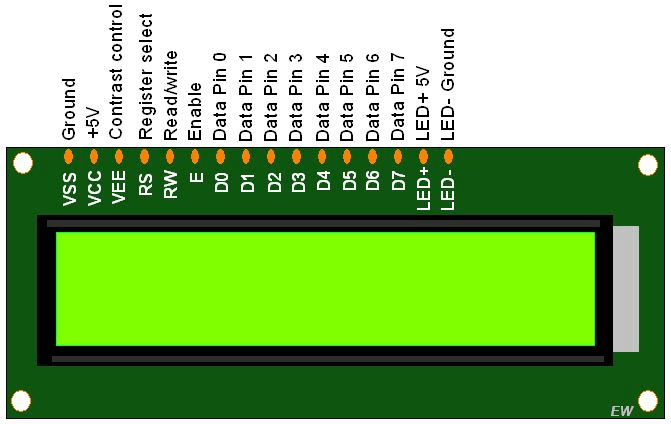
\includegraphics[width=0.5\linewidth]{1_LCD16x2_Pins.png}
    \caption{LCD Display}
    \label{fig:enter-label}
\end{figure}
\begin{figure}[H]
    \centering
    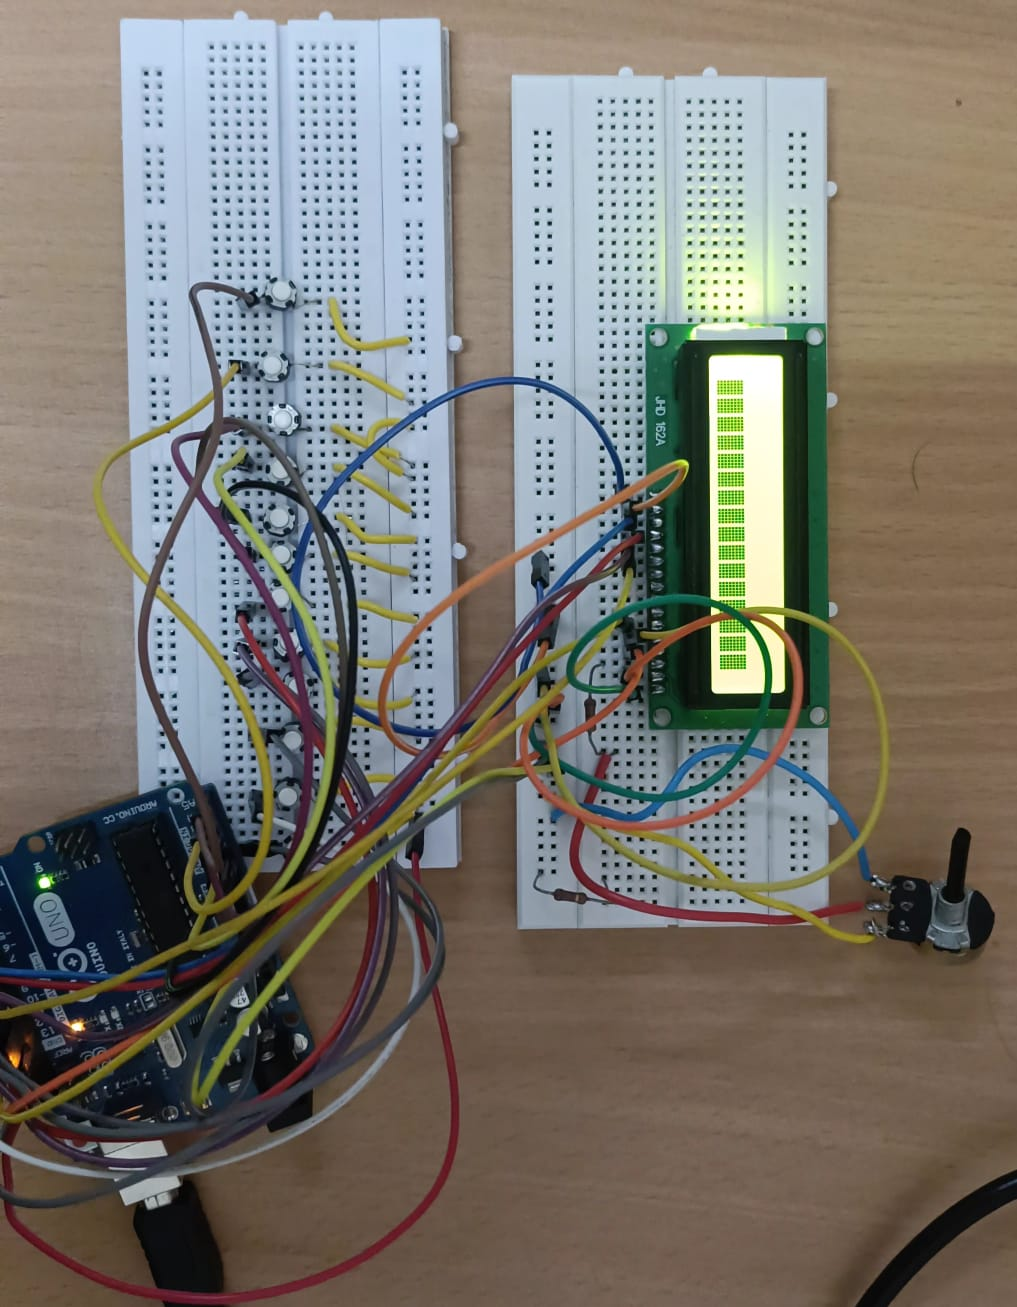
\includegraphics[width=0.5\linewidth]{WhatsApp Image 2025-03-24 at 19.40.29_df83bc3a.jpg}
    \caption{Hardware}
    \label{fig:enter-label}
\end{figure} 
\label{EndOfText}
\pagenumbering{arabic} 

\section{Working Explanation } \label{ch1}
\begin{itemize}
    \item \textbf{LCD Driver:}  
    \begin{itemize}
        \item Implemented in \texttt{lcd.h}, it includes functions such as:  
        \begin{itemize}
            \item \texttt{lcd\_init()}: Initializes the LCD.  
            \item \texttt{lcd\_clear()}: Clears the LCD display.  
            \item \texttt{lcd\_print()}: Prints a string or value on the LCD.  
        \end{itemize}
    \end{itemize}
    
    \item \textbf{Button Handling:}  
    \begin{itemize}
        \item Manages the detection of button presses, including numeric inputs (0-9) and special function keys.  
    \end{itemize}
    
    \item \textbf{Mathematical Evaluation:}  
    \begin{itemize}
        \item Utilizes a recursive descent parser for parsing arithmetic expressions.  
        \item Supports operations such as addition, subtraction, multiplication, and division.  
    \end{itemize}
    
    \item \textbf{Custom Mathematical Functions:}  
    \begin{itemize}
        \item Approximates trigonometric (\(\sin\), \(\cos\)) and logarithmic (\(\log\), \(\ln\)) functions using iterative methods.  
    \end{itemize}
\end{itemize}

\section*{Button Mapping and Modes}

Buttons facilitate numeric input and access various mathematical operations. The calculator operates in three modes:  

\begin{itemize}
    \item \textbf{Normal Mode:}  
    \begin{itemize}
        \item Allows entry of digits (0-9) and basic operations: \(+\), \(-\), \(*\), \(/\), \(=\), and \texttt{Backspace}.  
    \end{itemize}

    \item \textbf{Shift Mode:}  
    \begin{itemize}
        \item Provides access to advanced mathematical functions such as:  
        \begin{itemize}
            \item \(\sin\), \(\cos\), \(e^x\), and \(\sqrt{x}\).  
        \end{itemize}
    \end{itemize}

    \item \textbf{Extra Mode:}  
    \begin{itemize}
        \item Offers extended functionality with access to:  
        \begin{itemize}
            \item \(\arcsin\), \(\arccos\), \(\arctan\).  
            \item Logarithmic functions: \(\log\), \(\ln\).   
        \end{itemize}
    \end{itemize}
\end{itemize}
 
\label{EndOfText}
\label{endOfDoc}

\pagenumbering{arabic} 

\section{Code Outline $&$ Explanation } \label{ch1}

\definecolor{codebg}{rgb}{0.95,0.95,0.95}
\lstset{
    backgroundcolor=\color{codebg},
    basicstyle=\ttfamily\footnotesize,
    keywordstyle=\color{blue}\bfseries,
    commentstyle=\color{green!50!black},
    numbers=left,
    numberstyle=\tiny\color{gray},
    frame=single,
    breaklines=true
}
\subsection{Library Inclusions}
\begin{lstlisting}[language=C]
#include <avr/io.h>
#include <util/delay.h>
#include <stdlib.h>
#include <stdbool.h>
#include <string.h>
#include <ctype.h>
#include <math.h>
#include "lcd.h"
\end{lstlisting}
\textbf{Explanation:}
\begin{itemize}
\item \texttt{avr/io.h}: Provides access to microcontroller registers.
\item \texttt{util/delay.h}: Used for generating delays.
\item \texttt{stdbool.h}: Provides Boolean logic support.
\item \texttt{math.h}: Standard math library functions.
\item \texttt{lcd.h}: Custom LCD driver for display operations.
\end{itemize}

\subsection{Mathematical Functions Implementation}
Custom iterative approximations are used for trigonometric and logarithmic functions.

\subsubsection{Sine Approximation (Taylor Series)}
\begin{lstlisting}[language=C]
float mySin(float x){
float rad = x * PI / 180.0;
float term = rad;
float sum = rad;
for (int n = 1; n < 10; n++){
term = -term * rad * rad / ((2 * n) * (2 * n + 1));
sum += term;
}
return sum;
}
\end{lstlisting}
\subsubsection{Cos function}
\begin{lstlisting}[language=C]
float myCos(float x){
float rad = x * PI / 180.0;
float term = 1;
float sum = 1;
for (int n = 1; n < 10; n++){
    term = -term * rad * rad / ((2 * n - 1) * (2 * n));
    sum += term;
  }
  return sum;
}
\end{lstlisting}
\subsubsection{Square Root Function using Newton method}
\begin{lstlisting}[language=C]
float mySqrt(float x){
  if (x < 0) return -1;
  float guess = x / 2.0;
  for (int i = 0; i < 10; i++){
    guess = (guess + x / guess) / 2.0;
  }
  return guess;
}
\end{lstlisting}
\subsubsection{Natural logarithm}
\begin{lstlisting}[language=C]
float mySqrt(float x){
  if (x < 0) return -1;
  float guess = x / 2.0;
  for (int i = 0; i < 10; i++){
    guess = (guess + x / guess) / 2.0;
  }
  return guess;
}

}
\end{lstlisting}
\subsubsection{Exponential Approximation (Euler's Method)}
\begin{lstlisting}[language=C]
float myExp(float x){
int N = 100;
float h = x / N;
float y = 1.0;
for (int i = 0; i < N; i++){
y = y * (1 + h);
}
return y;
}
\end{lstlisting}

\subsection{Expression Parsing (Recursive Descent)}
Expressions are evaluated using a recursive descent parser.
\begin{lstlisting}[language=C]
float parseExpression(const char* s, int *pos) {
skipSpaces(s, pos);
float value = parseTerm(s, pos);
skipSpaces(s, pos);
while (s[*pos] == '+' || s[*pos] == '-') {
char op = s[(*pos)++];
float term = parseTerm(s, pos);
if (op == '+') value += term;
else value -= term;
skipSpaces(s, pos);
}
return value;
}
\end{lstlisting}

Parses and evaluates arithmetic expressions recursively.

\subsection{Button Handling}
Each button press is detected and processed accordingly.
\begin{lstlisting}[language=C]
bool button_pressed(uint8_t pinMask) {
return !(BUTTON_PORT & pinMask);
}
\end{lstlisting}

Checks if a button is pressed based on its pin state.

\subsection{LCD Update}
The LCD is updated with the current input string.
\begin{lstlisting}[language=C]
void updateLCD(void) {
lcd_clear();
lcd_print(input);
}
\end{lstlisting}

Clears and refreshes the display with new input.

\subsection{Main Execution Loop}
The program runs continuously, reading button inputs and updating the LCD.
\begin{lstlisting}[language=C]
int main(void) {
lcd_init();
lcd_clear();
lcd_print("Calculator Ready");
_delay_ms(1000);
lcd_clear();

while (1) {
// Read and process button inputs
updateLCD();
_delay_ms(10);
}
return 0;
}
\end{lstlisting}

Initializes the LCD and enters a loop to handle user inputs.
\newpage 
\label{EndOfText}
\label{endOfDoc}

\pagenumbering{arabic} 

\section{Conclusion} \label{ch1}
This project successfully implements a scientific calculator for the AVR microcontroller, allowing users to input expressions via buttons and view results on an LCD display. The key features include:
\begin{itemize}
\item Support for basic arithmetic and advanced mathematical functions.
\item A recursive descent parser for accurate expression evaluation.
\item Custom approximations for trigonometric, logarithmic, and exponential functions.
\end{itemize}

Future enhancements could include:
\begin{itemize}
\item Improving numerical accuracy by increasing iterations in Taylor series expansions.
\item Expanding functionality to include additional mathematical functions.
\item Optimizing memory usage for improved performance on low-memory microcontrollers.
\end{itemize} 
\label{EndOfText}
\label{endOfDoc}

\pagenumbering{arabic} 

\section{References} \label{ch1}
\input{sources/references} 
\label{EndOfText}
\label{endOfDoc}
\end{document}
